%\section{Hadamard and S Gates}

\label{subsection:logical}
The $\rotfvs{}$ notation gives a nice interpretation of the logical code words. Particularly, an $X$-type logical codeword is given as follows: Take a subset of generators $S^{\prime} \subset S$ and consider the subgroup generated by it, $\expval*{S^{\prime}}$; let us denote the subgroup by $K$. Then the logical codeword is the $X$-product over all $\rotfv{u}{S^{\prime}}$ such that $u \in K$. Moreover, replacing $K$ by a coset whose base subgroup is $\expval*{S^{\prime}}$, we get another presentation of the same logical codeword.
\begin{claim}
  For any generator subset $S^{\prime}$ of size $d^{\prime}$, denote by $x_{S^{\prime}}$ and $z_{S^{\prime}}$ the following $d^{\prime}$-dimensional chains: 
\begin{equation*}
  \begin{split}
    x_{S^{\prime}}  \colonequals \sum_{u \in \expval*{S^{\prime}} }\rotfv{u}{S^{\prime}} \ \ \ z_{S^{\prime}} \colonequals \sum_{u \in \expval*{S/S^{\prime}} }\rotfv{u}{S^{\prime}} 
  \end{split}
\end{equation*}
Then $x_{S^{\prime}}$ and $z_{S^{\prime}}$ are binary representations of anticommuting logical codewords of the $(d,d^{\prime})$-Toric code. In particular, $x_{S^{\prime}} \in \mathcal{C}_{X}/\mathcal{C}_{Z}^{\perp}$, $z_{S^{\prime}} \in \mathcal{C}_{Z}/\mathcal{C}_{X}^{\perp}$, and $x_{S^{\prime}} z_{S^{\prime}} = 1$. In addition, let $X_{S^{\prime}}$ and $Z_{S^{\prime}}$ be the Pauli matrices obtained by multiplying each non-trivial coordinate of them by $X$ or $Z$, respectively.
\end{claim}
\begin{proof}
By definition, $x_{S^{\prime}}$ and $z_{S^{\prime}}$ are binary assignments on the $d^{\prime}$-dimensional faces. We start by showing that $x_{S^{\prime}} \in \mathcal{C}_{X}$ and $z_{S^{\prime}} \in \mathcal{C}_{Z}$; namely, that the boundaries $\partial^{-}x_{S^{\prime}}$ and $\partial^{+}z_{S^{\prime}}$ vanish.
\begin{equation*}
  \begin{split}
    \partial^{-} \sum_{u \in \expval*{S^{\prime}} }\rotfv{u}{S^{\prime}} &=  \sum_{u \in \expval*{S^{\prime}} } \sum_{g\in S^{\prime}} \rotfv{ u}{S^{\prime}/g} +  \rotfv{gu}{S^{\prime}/g} \\
     &=  \sum_{g\in S^{\prime}} \sum_{u \in \expval*{S^{\prime}} } \rotfv{ u}{S^{\prime}/g} +  \sum_{u \in \expval*{S^{\prime}} }\rotfv{gu}{S^{\prime}/g} \\
     &=  \sum_{g\in S^{\prime}} \sum_{u \in \expval*{S^{\prime}} } \rotfv{ u}{S^{\prime}/g} +  \sum_{u \in \expval*{S^{\prime}} }\rotfv{u}{S^{\prime}/g} = 0 
  \end{split}
\end{equation*}
\begin{equation*}
  \begin{split}
    \partial^{+} \sum_{u \in \expval*{S^{\prime}} }\rotfv{u}{S/S^{\prime}} &=  \sum_{u \in \expval*{S^{\prime}} } \sum_{g\in S^{\prime}} \rotfv{ u}{S/S^{\prime} \cup g} +  \rotfv{g^{-1} u}{S/S^{\prime} \cup g} \\
    &=  \sum_{g\in S^{\prime}} \sum_{u \in \expval*{S^{\prime}} } \rotfv{ u}{S/S^{\prime} \cup g} +  \sum_{u \in \expval*{S^{\prime}} }\rotfv{g^{-1}u}{S/S^{\prime}\cup g} \\
     &=  \sum_{g\in S^{\prime}} \sum_{u \in \expval*{S^{\prime}} } \rotfv{ u}{S/S^{\prime}\cup g} +  \sum_{u \in \expval*{S^{\prime}} }\rotfv{u}{S/S^{\prime} \cup g} = 0 
  \end{split}
\end{equation*}
Thus $x_{S^{\prime}} \in \mathcal{C}_{X}$ and $z_{S^{\prime}}\in \mathcal{C}_{Z}$, now for showing that they are not binary representations of stabilizers, it's enough to show they admit no vanishing product.  
\begin{equation*}
  \begin{split}
    x_{S^{\prime}}z_{S^{\prime}} = \sum_{u \in \expval*{S^{\prime}} }\rotfv{u}{S^{\prime}} \sum_{u \in \expval*{S/S^{\prime}} }\rotfv{u}{S^{\prime}} = \rotfv{e}{S^{\prime}} \rotfv{e}{S^{\prime}} = 1
  \end{split}
\end{equation*}
Therefore, the Paulis $X_{S^{\prime}}$ and $Z_{S^{\prime}}$ are $X$- and $Z$-type anticommuting logical code words.
\end{proof}


\input{./tikz/logical-toric.tikz}
The $(d,d^{\prime})$-Toric code admits a fold-transversal Hadamard-type realization for any dimensions $d,d^{\prime}$. Particularly, the gate exchanges logical Pauli $X_{S^{\prime}}$ with logical Pauli $Z_{S/S^{\prime}}$ and vice versa. It is realized by an application of transversal Hadamards followed by permuting the qubits according to a transformation which we name the \textit{$\phi$-transpose map}. We define the transpose map as follows:
\begin{definition}[The Transpose Map]
  Let $d, d^{\prime}$ be integers, such that $d^{\prime} < d$, and let $\mathcal{G}$ be a $(d, d^{\prime})$-Toric complex generated by the generator set $S$.  Let us define the multiplication of geneerators subset $S^{\prime}\subset S$ by a vertex $v \in V(\mathcal{G})$ as follows: 
  \begin{equation*}
    \begin{split}
      S^{\prime} v = \left(\prod_{g \in S^{\prime}}g^{\prime} \right) v
    \end{split}
  \end{equation*}
  We define the \textit{transpose map} $\phi : \mathcal{F}^{d^{\prime}} \rightarrow \mathcal{F}^{d - d^{\prime}}$ by acting on the basis elements as follows:
  \begin{equation*}
    \begin{split}
      \phi(\rotfv{v}{S^{\prime}}) \rightarrow \rotfv{ S^{\prime}v }{S/S^{\prime}} 
    \end{split}
  \end{equation*}
\end{definition}
Notice that the transpose map is a permutation over the bits and therefore can be realized at constant depth. 
\begin{definition}[ Hadamard-Type Gate $\mathbf{H_{\phi}}$]  
  We define the logical Hadamard-type gate $ \mathbf{H_{\phi}} \colon L (\mathcal{H}) \rightarrow L (\mathcal{H}) $ as follows, for any $ S' \subset S $, of size $ d' $:
  \begin{equation*}
    \begin{split}
      \mathbf{H_{\phi}} ( X_{S^{\prime}} )  \rightarrow Z_{S/S^{\prime}} \ \ \ \  \mathbf{H_{\phi}} ( Z_{S^{\prime}} )   \rightarrow X_{S/S^{\prime}} 
    \end{split}
  \end{equation*}
\end{definition}
\begin{claim}
  The Hadamard-type gate $ \mathbf{H_{\phi}}$ has a fold-transversal implementation by, first applying $\mathbf{H}^{n}$ over all the physical qubits, and then permuting them by the transpose map $\phi$, namely $\mathbf{\hat{H}}_{\phi} = \phi \circ \mathbf{H}^{n}$.
\end{claim}
\begin{proof}
  Clearly, for any subset of generators $S^{\prime} \subset S$, the map $\phi$ sends $x_{S^{\prime}}$ to $z_{S/S^{\prime}}$:
  \begin{equation*}
    \begin{split}
    \phi(x_{S^{\prime}}) = \phi(  \sum_{u \in \expval*{S^{\prime}} }\rotfv{u}{S^{\prime}}   ) =  \sum_{u \in \expval*{S^{\prime}} }\rotfv{ S^{\prime} u}{S/S^{\prime}}  = \sum_{u \in \expval*{S^{\prime}} }\rotfv{u}{S/S^{\prime}} = z_{S/S^{\prime}}
    \end{split}
  \end{equation*}
Moreover, $\phi$ sends binary representations of $Z$-stabilizers to binary representations of $X$-stabilizers, and vice versa. To see this, consider a $d^{\prime}+1$ dimensional face, and consider the image of the stabilizer it defines.
  \begin{equation*}
    \begin{split}
      \phi \left( \partial^{-}  \rotfv{v}{S^{\prime}} \right) &=  \phi\left( \sum_{g\in S^{\prime}} \rotfv{v}{S^{\prime}/g} +  \rotfv{gv}{S^{\prime}/g}  \right) \\
      & = \sum_{g\in S^{\prime}} \rotfv{ g^{-1}  S^{\prime} v}{(S/S^{\prime})\cup g} +  \rotfv{ g^{-1} S^{\prime}  gv}{(S/S^{\prime})\cup g}  \\ 
      &= \partial^{+} \rotfv{ S^{\prime} v}{S/S^{\prime}}
    \end{split}
  \end{equation*}
  And for the checks set on the $d^{\prime}-1$-dimensional face we have: 
  \begin{equation*}
    \begin{split}
      \phi \left( \partial^{+}  \rotfv{v}{S/S^{\prime}} \right) & =   \phi \left( \sum_{g \in S^{\prime}}\rotfv{ g^{-1} v}{(S/S^{\prime}) \cup g} +   \rotfv{    v}{(S/S^{\prime}) \cup g} \right) \\
      &=  \sum_{g \in S^{\prime}}\rotfv{  (S/S^{\prime})    v}{S^{\prime}/g} +   \rotfv{   g (S/S^{\prime})  v}{S^{\prime} / g} \\
      & =  \partial^{-} \rotfv{ (S/S^{\prime}) v}{S^{\prime}}
    \end{split}
  \end{equation*}
  Thus, $\mathbf{H}^{\otimes n} \circ \phi$ sends $Z$-stabilizers to $X$-stabilizers and vice versa, thereby preserving the code space. Combining this with the above, $\mathbf{H}^{\otimes n} \circ \phi$ realizes the logical gate $\mathbf{H}_{\phi}$ in the $(d,d^{\prime})$-Toric code.
\end{proof}

    \begin{figure}[h]

\begin{center}
    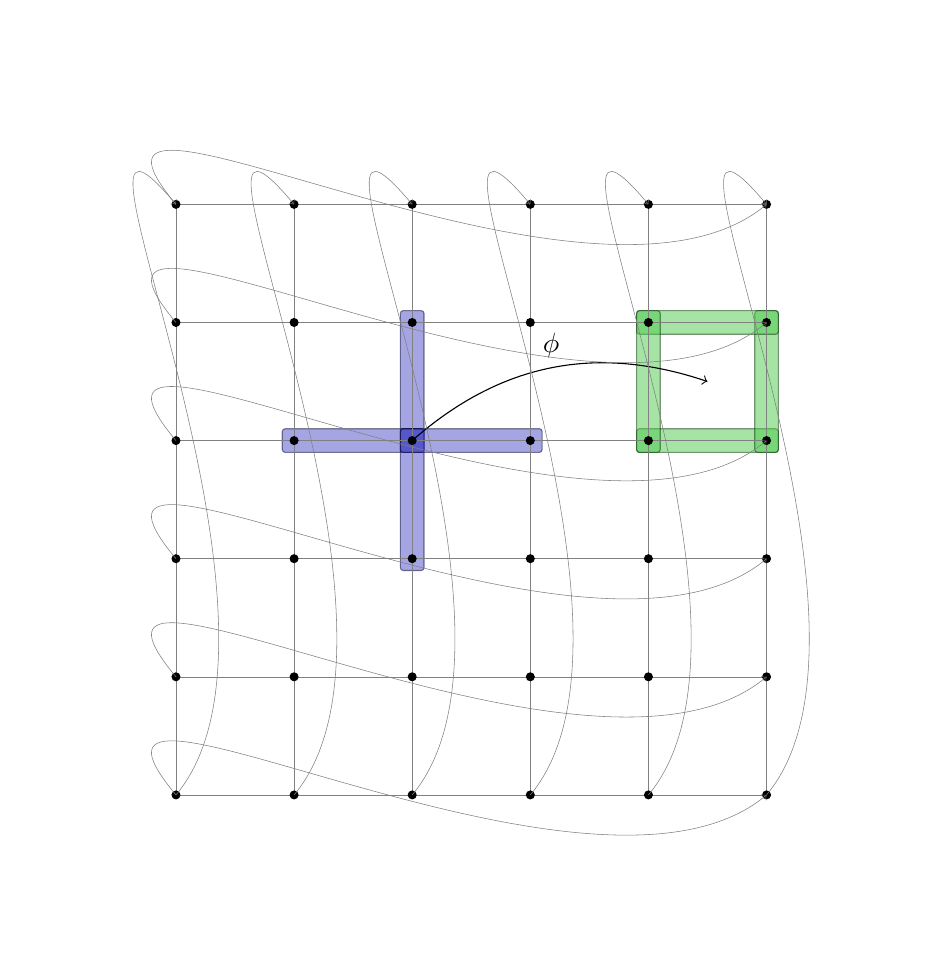
\begin{tikzpicture}[scale=1.5]


  %\draw[blue!20!black,fill=blue!70!black!70,rounded corners=1]%shift={(0.15,0.15)}]
  %(0.9,-0.1) node[below] {$\rotfv{v}{\{ g_{1}\} } $}
  %rectangle (1.1,1.1);


  \draw[blue!20!black,fill=blue!70!black!70,rounded corners=1, opacity=0.5]%,shift={(0.15,0.15)}]
  (1.9,2.9) rectangle (2.1,4.1);
  \draw[blue!20!black,fill=blue!70!black!70,rounded corners=1, opacity=0.5]%,shift={(0.15,0.15)}]
  (0.9,2.9) rectangle (2.1,3.1);
  \draw[blue!20!black,fill=blue!70!black!70,rounded corners=1, opacity=0.5]%,shift={(0.15,0.15)}]
  (1.9,1.9) rectangle (2.1,3.1);
  \draw[blue!20!black,fill=blue!70!black!70,rounded corners=1, opacity=0.5]%,shift={(0.15,0.15)}]
  (1.9,2.9) rectangle (3.1,3.1);



  \draw[green!20!black,fill=green!70!black!70,rounded corners=1, opacity=0.5]%,shift={(0.15,0.15)}]
  (3.9,2.9) rectangle (5.1,3.1);
  \draw[green!20!black,fill=green!70!black!70,rounded corners=1, opacity=0.5]%,shift={(0.15,0.15)}]
  (4.9,2.9) rectangle (5.1,4.1);
  \draw[green!20!black,fill=green!70!black!70,rounded corners=1, opacity=0.5]%,shift={(0.15,0.15)}]
  (3.9,3.9) rectangle (5.1,4.1);
  \draw[green!20!black,fill=green!70!black!70,rounded corners=1, opacity=0.5]%,shift={(0.15,0.15)}]
  (3.9,2.9) rectangle (4.1,4.1);


  \draw[black,->, bend left]  (2,3) to node[midway, above]{ $\phi$ } (4.5,3.5) ;

%  \draw[blue!20!black,fill=blue!70!black!70,rounded corners=1]%,shift={(0.15,0.15)}]
%  (3.9,2.9) rectangle (3.1,3.1);
%  \draw[blue!20!black,fill=blue!70!black!70,rounded corners=1]%,shift={(0.15,0.15)}]
%  (3.9,1.9) rectangle (3.1,2.1);
%  \draw[blue!20!black,fill=blue!70!black!70,rounded corners=1]%,shift={(0.15,0.15)}]
%  (3.9,0.9) rectangle (3.1,1.1);
%  \draw[blue!20!black,fill=blue!70!black!70,rounded corners=1]%,shift={(0.15,0.15)}]
%  (3.9,3.9) rectangle (3.1,4.1);
  %\draw[blue!20!black,fill=blue!70!black!70,rounded corners=1]%,shift={(0.15,0.15)}]
  %(3.9,4.9) rectangle (3.1,1.1);
 % \draw[blue!20!black,fill=blue!70!black!70,rounded corners=1]%,shift={(0.15,0.15)}]
  %(3.9,-0.1) rectangle (3.1,0.1);


  \draw[step=1cm,gray,very thin] (0,0) grid (5,5);
  \foreach \x in {0,1,2,3,4,5}
  \foreach \y in {0,1,2,3,4,5}
  {
  \node[draw,circle,inner sep=1pt,fill] at (\x,\y) {};
}
\draw[gray,very thin,-> ]  (0,0) to [out=50, in=130] (0,5);
\draw[gray,very thin,-> ]  (1,0) to [out=50, in=130] (1,5);
\draw[gray,very thin,-> ]  (2,0) to [out=50, in=130] (2,5);
\draw[gray,very thin,-> ]  (3,0) to [out=50, in=130] (3,5);
\draw[gray,very thin,-> ]  (4,0) to [out=50, in=130] (4,5);
\draw[gray,very thin,-> ]  (5,0) to [out=50, in=130] (5,5);
\draw[gray,very thin,-> ]  (0,5) to [out=130, in=220] (5,5);
\draw[gray,very thin,-> ]  (0,4) to [out=130, in=220] (5,4);
\draw[gray,very thin,-> ]  (0,3) to [out=130, in=220] (5,3);
\draw[gray,very thin,-> ]  (0,2) to [out=130, in=220] (5,2);
\draw[gray,very thin,-> ]  (0,1) to [out=130, in=220] (5,1);
\draw[gray,very thin,-> ]  (0,0) to [out=130, in=220] (5,0);


\end{tikzpicture}
\end{center}
\caption{On the left is the Toric Graph. On the right are cross and face checks.}
\label{fig:transposeToric}
\end{figure}

 

\begin{definition}
Let $\psi \colon S \rightarrow S$ be a permutation on the generators in $S$, so $\psi$ has a natural extension to an automorphism on $\mathcal{G}$\footnote{By replacing each of the generators in a product by its image according to $\psi$.}. Extend $\psi$ to act over the faces of the $(d,d^{\prime})$-Toric as follows:
  \begin{equation*}
    \begin{split}
      \psi( \rotfvs{}) \colonequals \rotfv{\psi(v)}{\psi(S^{\prime})}
    \end{split}
  \end{equation*}
  We name the map a $\psi$-permutation. 
\end{definition}

\begin{claim}
The $\psi$-permutation sends $X$-checks to $X$-checks and $Z$-checks to $Z$-checks. Moreover, assume that $d^{\prime}=d/2$. Then, for a generator subset $J\subset S$ such that $d^{\prime} = |J| = |S/J|$ and $S/J = \psi(J)$, we have that the application of $\psi$ realizes the exchange $x_{J} \leftrightarrow x_{S/J}$.
\end{claim}

\begin{proof}
     
  \begin{equation*}
    \begin{split}
      \psi \left( \partial^{-} \rotfvs{} \right) &= \psi \left( \sum_{g\in S^{\prime}} \rotfv{v}{S^{\prime}/g} + \rotfv{gv}{S^{\prime}/g}   \right) \\
      &= \sum_{g\in S^{\prime}} \rotfv{ \psi(v)}{\psi(S^{\prime})/\psi(g)} + \rotfv{\psi(g)\psi(v)}{\psi(S^{\prime})/\psi(g)}  \\
      &= \sum_{g\in S^{\prime}} \rotfv{ \psi(v)}{\psi(S^{\prime})/g} + \rotfv{g\psi(v)}{\psi(S^{\prime})/g}  \\
      &= \partial^{-}\rotfv{\psi(v)}{\psi(S^{\prime})}
    \end{split}
  \end{equation*}
Since $\psi$ is a permutation over $S$, it follows that $|\psi(S^{\prime})| = |S^{\prime}| = d^{\prime} + 1$; namely, $\partial^{-}\rotfv{\psi(v)}{\psi(S^{\prime})}$ is a $Z$-check. The same calculation shows that for $S^{\prime}$ at size $|S^{\prime}|=d^{\prime}-1$, we have $\psi \left( \partial^{+} \rotfvs{} \right) = \partial^{+}\rotfv{\psi(v)}{\psi(S^{\prime})}$. 

Now, consider $J\subset S$ such $|J|=d^{\prime}$ and $\psi(J) = S/J$. Then: 
\begin{equation*}
  \begin{split}
    \psi(x_{J}) =  \psi \left( \sum_{v \in \expval*{J}} \rotfv{v}{J} \right) = \sum_{v \in \expval*{J}} \rotfv{\psi(v)}{\psi(J)} = \sum_{v \in \expval*{S/J}} \rotfv{v}{S/J} 
  \end{split}
\end{equation*}
Where we used the fact that $\psi$ sends the group generated by $J$ to the group generated by the complement generator set. Since $\psi$ is a permutation, $\psi(S/J) = J$, and therefore $\psi(x_{S/J}) = x_J$.
\end{proof}

\begin{corollary}
For $ d' = d - d' = d/2 $, one can fix a generator subset $ S' $ of size $|S'|$, and realize a Hadamard gate that exchanges $ X_{S'} \leftrightarrow Z_{S'} $.
\end{corollary}



Equipped with $\mathbf{H}_{\phi}$, we gain a mapping into the dual code that both keeps the Toric skeleton and sends the $Z$-checks to $d^{\prime}-1$ dimensional faces. Later (in \Cref{subsection:dualcode}), this will be advantageous, enabling the use of the same local decoder (with a slight change) to act on both $\mathcal{C}_{X}$ and its dual. 


Throughout the construction, we encode each qubit in a code block; namely, we restrict ourselves to using only a single codeword of the $(d,d^{\prime})$-Toric code. From now on, we will think of $S^{\prime} \subset S$ as a fixed $d^{\prime}$-size subset of generators that were picked from the head. And we will decode the logical $\ket{1}$ state by $x_{S^{\prime}}$. To simplify terminology, we call such usage 'nice encoding'.
\begin{definition}[The Nice Encoding]
  Consider $(d,d^{\prime})$-Toric code and fix a subset $S^{\prime} \subset S$, at size $d^{\prime}$. We define the \textit{nice encoding} to be the subsystem code, which uses $x_{S^{\prime}}$ to encode a single logical qubit. Namely, the logical codewords are: 
  \begin{equation*}
    \begin{split}
      \ket{ \bar{0} } &= \ket{ \mathcal{C}_{Z}^{\perp} } \\ 
      \ket{ \bar{1} } &= \ket{ x_{S^{\prime}} + \mathcal{C}_{Z}^{\perp} } 
    \end{split}
  \end{equation*}
\end{definition}
We are now ready to give a full description of the realization of the logical operators. The logical Paulis $X$ and $Z$ are realized by the application of $X_{S^{\prime}}$ and $Z_{S^{\prime}}$. For the gates $\mathbf{S}$ and $\mathbf{T}$, we use single-qubit gate teleportation as presented in \Cref{fig:magic}. In single-qubit gate teleportation, the resource $\ket{\mathbf{S}}$ is initialized as $\mathbf{S}\ket{+}$, similarly for $\ket{\mathbf{T}}$. The gate $\mathbf{1}_{S^{\prime}}$ stands for the classical procedure that, given the measurement results, checks whether the logical bit $\ket{1}$ is turned on. We will return to this gate with a higher resolution depiction of it after the description of the Hadamard teleportation.
    \begin{figure}[h]
        \centering 
        \begin{quantikz}
          \lstick{$\ket{\psi}$} & \ctrl{1}  &  & \gate{Z_{S^{\prime}}} &  \rstick{$\mathbf{S}\ket{\psi}$} \\
        \lstick{$\ket{\mathbf{S}}$} & \targ{} & \meter{} &  \gate{\mathbf{1}_{x_{S^{\prime}}}} \wire[u][1]{c}    \\
        \end{quantikz} \qquad \qquad 
        \begin{quantikz}
          \lstick{$\ket{\psi}$} & \ctrl{1}  & & \gate{\mathbf{S}} &  \rstick{$\mathbf{T}\ket{\psi}$} \\
          \lstick{$\ket{\mathbf{T}}$} & \targ{} & \meter{} & \gate{\mathbf{1}_{x_{S^{\prime}}}} \wire[u][1]{c}    \\
        \end{quantikz}
        \caption{ Simulating the $\mathbf{S}$ and $\mathbf{T}$ gates, using the $\ket{\mathbf{S}}$, $\ket{\mathbf{T}}$ magic states. }   
\label{fig:magic}
\end{figure}


For the Hadamard gate, we use a modification of the standard two-qubit gate teleportation as shown in \Cref{fig:magich}. The realization differs from the standard realization as the measurement in the phase basis is done by first moving to the dual space via the application of physical $\mathbf{H}^{\otimes n}$, measuring, reorganizing the qubits through $\phi$, and then checking for the $x_{S/S^{\prime}}$ outcome (thus, it can be thought of as the application of $\mathbf{H}_{\phi}$ and then measurement). In addition, unlike the single-qubit gate teleportation, here $\ket{\mathbf{H}}$ is initialized as $I\otimes H (\ket{00} + \ket{11})$ (up to normalization).
    \begin{figure}[h]
        \centering 
        \begin{quantikz}
          \lstick{$\ket{\psi}$} & \ctrl{1}  & \gate{\mathbf{H}^{\otimes n}} & \meter{} \wire{c} & \gate{ \phi } &  \gate{\mathbf{1}_{x_{S/S^{\prime}}}} \wire[d][2]{c} \\
         \lstick[2]{$\ket{\mathbf{H}}$} & \targ{} & & \meter{} &   \gate{\mathbf{1}_{x_{S^{\prime}}}} \wire[d][1]{c}   \\
         & &  & & \gate{Z_{S^{\prime}}}   & \gate{X_{S^{\prime}}}  & \rstick{$\mathbf{H}\ket{\psi}$} \\
        \end{quantikz} 
        \caption{Gate teleportation of the Hadamard gate, using the resource $\ket{\mathbf{H}}$. We emphasize again that although the Hadamard (at least Hadamard-type) has an $O(1)$-depth gate realization, we still need all the operations on the quantum register to be strictly transversal for the sake of the proof. Thus, we realize the Hadamard via gate teleportation. }   
\label{fig:magich}
\end{figure}


The classical procedure of logical codeword checking, namely $ \mathbf{1}_{x_{S^{\prime}}}$ / $ \mathbf{1}_{x_{S/S^{\prime}}}$, is divided into four stages. In the first, we find all the deviation clusters of the Tanner graph. This requires finding connected components, which is known to be done in $\log^{2}(n)$ depth (See \cite{SHILOACH198257} and \cite{1676869} for logarithmic time connected components in the PRAM model and \cite{Lev1980} for the simulation of PRAM machines using bounded-fan circuits). Then, we broadcast the connected components. Conceptually, each deviation cluster is sent to its own register; technically, we copy the restriction of the syndromes to the deviation cluster. The broadcast also requires at most $\log(n)$ depth since there can be at most \#checks $=\Theta(n)$ deviation clusters and therefore at most $\Theta(n)$ copies. Then, we decode each of the copies in parallel. The separation of the clusters guarantees that during decoding, clusters will not merge into a larger cluster. For the decoding, we iterate sweep-rule cycles (defined in \Cref{def:sweeprule}) until erasing the syndrome. Later, we will see that the decoding depth is bounded by $\Theta(n)$ (See \Cref{col:idealcorrection}). Finally, we combine the results of all the decoding sessions together by Xoring their correction suggestions. Each of the Xor operations is between at most $n$ qubits and therefore requires at most $\log(n)$ depth. So the overall depth for performing a logical measurement is $\Theta(n)$. The additional classical width consists of restricting the syndrome for each of the deviation clusters. We will store them as check assignments $\mathbb{F}_{2}^{\mathcal{F}_{d^{\prime} -1} }$, namely an addition of $\Theta(n)$ bits per deviation cluster and in total $\Theta(n^{2})$.



%
%Next, we are going to provide a reliztion of the logical measurment in the phase base, where the the application of 
%For now, we are fine, with stating a corollary, suppose that we have a single-shot decoder $D$ that 

%logical Hadamard gate can be realizied by permuting th
%We emphiss that although $\mathbf{H}_{\phi}$ is not equevalnce to $\mathbf{
%\begin{corollary}
%There is a realization of $\mathcal{C}_{X}/\mathcal{C}_{Z}^{\perp} \rightarrow \mathcal{C}_{Z}/\mathcal{C}_{X}^{\perp}$ that keeps the structure of the Toric skeleton.
%\end{corollary}
%\ctt{Change the definition above such that it will be about moving to the dual code $\mathcal{C}_{X}/\mathcal{C}_{Z}^{\perp} \rightarrow \mathcal{C}_{Z}/\mathcal{C}_{X}^{\perp}$. And not about the logical Hadamard. }
%\ctt{  Here, add that the measurement in the $X$-basis can be done using $\textbf{H}^{n}$, measurement,  and then $\log(n)$ classical depth. }









